% ============================================================
% Question Bank: ch03-09 Introduction to Square Roots
% Topic Title: Introduction to Square Roots
% CCSS: Supplementary
% Questions: 30 (18 MC + 7 SA + 5 Graphical)
% ============================================================

% --- Multiple Choice Questions (18) ---

\begin{practiceQuestion}{3-9-q01}{mc}
\begin{questionText}
What is $\sqrt{49}$?
\end{questionText}
\choiceA{$6$}
\choiceB{$7$}
\choiceC{$8$}
\choiceD{$24.5$}
\correctAnswer{B}
\explanation{$7 \times 7 = 49$, so $\sqrt{49} = 7$.}
\end{practiceQuestion}

\begin{practiceQuestion}{3-9-q02}{mc}
\begin{questionText}
What is $\sqrt{144}$?
\end{questionText}
\choiceA{$11$}
\choiceB{$12$}
\choiceC{$13$}
\choiceD{$72$}
\correctAnswer{B}
\explanation{$12 \times 12 = 144$, so $\sqrt{144} = 12$.}
\end{practiceQuestion}

\begin{practiceQuestion}{3-9-q03}{mc}
\begin{questionText}
Which number is a perfect square?
\end{questionText}
\choiceA{$18$}
\choiceB{$24$}
\choiceC{$36$}
\choiceD{$50$}
\correctAnswer{C}
\explanation{$36 = 6 \times 6$. The other numbers cannot be written as an integer times itself.}
\end{practiceQuestion}

\begin{practiceQuestion}{3-9-q04}{mc}
\begin{questionText}
Between which two whole numbers is $\sqrt{30}$?
\end{questionText}
\choiceA{$4$ and $5$}
\choiceB{$5$ and $6$}
\choiceC{$6$ and $7$}
\choiceD{$7$ and $8$}
\correctAnswer{B}
\explanation{$25 < 30 < 36$, so $5 < \sqrt{30} < 6$.}
\end{practiceQuestion}

\begin{practiceQuestion}{3-9-q05}{mc}
\begin{questionText}
What is $\sqrt{100}$?
\end{questionText}
\choiceA{$10$}
\choiceB{$50$}
\choiceC{$25$}
\choiceD{$20$}
\correctAnswer{A}
\explanation{$10 \times 10 = 100$, so $\sqrt{100} = 10$.}
\end{practiceQuestion}

\begin{practiceQuestion}{3-9-q06}{mc}
\begin{questionText}
Which is the best estimate for $\sqrt{20}$?
\end{questionText}
\choiceA{$4.0$}
\choiceB{$4.5$}
\choiceC{$5.0$}
\choiceD{$10.0$}
\correctAnswer{B}
\explanation{$16 < 20 < 25$, so $4 < \sqrt{20} < 5$. Since $20$ is near the middle, $\sqrt{20} \approx 4.5$.}
\end{practiceQuestion}

\begin{practiceQuestion}{3-9-q07}{mc}
\begin{questionText}
A square has an area of $64$ square inches. What is the side length?
\end{questionText}
\choiceA{$4$ in}
\choiceB{$16$ in}
\choiceC{$8$ in}
\choiceD{$32$ in}
\correctAnswer{C}
\explanation{Side $= \sqrt{64} = 8$ inches because $8 \times 8 = 64$.}
\end{practiceQuestion}

\begin{practiceQuestion}{3-9-q08}{mc}
\begin{questionText}
Which of the following is NOT a perfect square?
\end{questionText}
\choiceA{$81$}
\choiceB{$121$}
\choiceC{$150$}
\choiceD{$169$}
\correctAnswer{C}
\explanation{$81 = 9^2$, $121 = 11^2$, $169 = 13^2$. But $150$ is not a perfect square.}
\end{practiceQuestion}

\begin{practiceQuestion}{3-9-q09}{mc}
\begin{questionText}
What is $\sqrt{1}$?
\end{questionText}
\choiceA{$0$}
\choiceB{$1$}
\choiceC{$-1$}
\choiceD{Undefined}
\correctAnswer{B}
\explanation{$1 \times 1 = 1$, so $\sqrt{1} = 1$.}
\end{practiceQuestion}

\begin{practiceQuestion}{3-9-q10}{mc}
\begin{questionText}
Between which two whole numbers is $\sqrt{75}$?
\end{questionText}
\choiceA{$7$ and $8$}
\choiceB{$8$ and $9$}
\choiceC{$9$ and $10$}
\choiceD{$6$ and $7$}
\correctAnswer{B}
\explanation{$64 < 75 < 81$, so $8 < \sqrt{75} < 9$.}
\end{practiceQuestion}

\begin{practiceQuestion}{3-9-q11}{mc}
\begin{questionText}
What is $\sqrt{0}$?
\end{questionText}
\choiceA{$0$}
\choiceB{$1$}
\choiceC{Undefined}
\choiceD{$-1$}
\correctAnswer{A}
\explanation{$0 \times 0 = 0$, so $\sqrt{0} = 0$.}
\end{practiceQuestion}

\begin{practiceQuestion}{3-9-q12}{mc}
\begin{questionText}
Which is the best estimate for $\sqrt{50}$?
\end{questionText}
\choiceA{$6.5$}
\choiceB{$7.1$}
\choiceC{$7.5$}
\choiceD{$8.0$}
\correctAnswer{B}
\explanation{$49 < 50 < 64$, so $7 < \sqrt{50} < 8$. Since $50$ is very close to $49$, $\sqrt{50} \approx 7.1$.}
\end{practiceQuestion}

\begin{practiceQuestion}{3-9-q13}{mc}
\begin{questionText}
A square garden has an area of $196$ ft$^2$. What is the perimeter?
\end{questionText}
\choiceA{$14$ ft}
\choiceB{$49$ ft}
\choiceC{$56$ ft}
\choiceD{$784$ ft}
\correctAnswer{C}
\explanation{Side $= \sqrt{196} = 14$ ft. Perimeter $= 4 \times 14 = 56$ ft.}
\end{practiceQuestion}

\begin{practiceQuestion}{3-9-q14}{mc}
\begin{questionText}
What is $\sqrt{225}$?
\end{questionText}
\choiceA{$12$}
\choiceB{$13$}
\choiceC{$14$}
\choiceD{$15$}
\correctAnswer{D}
\explanation{$15 \times 15 = 225$, so $\sqrt{225} = 15$.}
\end{practiceQuestion}

\begin{practiceQuestion}{3-9-q15}{mc}
\begin{questionText}
Which two perfect squares does $110$ fall between?
\end{questionText}
\choiceA{$81$ and $100$}
\choiceB{$100$ and $121$}
\choiceC{$121$ and $144$}
\choiceD{$64$ and $81$}
\correctAnswer{B}
\explanation{$100 = 10^2$ and $121 = 11^2$. Since $100 < 110 < 121$, $\sqrt{110}$ is between $10$ and $11$.}
\end{practiceQuestion}

\begin{practiceQuestion}{3-9-q16}{mc}
\begin{questionText}
If $n^2 = 169$, what is $n$ (assuming $n > 0$)?
\end{questionText}
\choiceA{$11$}
\choiceB{$12$}
\choiceC{$13$}
\choiceD{$14$}
\correctAnswer{C}
\explanation{$13 \times 13 = 169$, so $n = 13$.}
\end{practiceQuestion}

\begin{practiceQuestion}{3-9-q17}{mc}
\begin{questionText}
Which is the best estimate for $\sqrt{90}$?
\end{questionText}
\choiceA{$8.5$}
\choiceB{$9.0$}
\choiceC{$9.5$}
\choiceD{$10.0$}
\correctAnswer{C}
\explanation{$81 < 90 < 100$, so $9 < \sqrt{90} < 10$. Since $90$ is close to $81$, $\sqrt{90} \approx 9.5$.}
\end{practiceQuestion}

\begin{practiceQuestion}{3-9-q18}{mc}
\begin{questionText}
What is $\sqrt{4} + \sqrt{9}$?
\end{questionText}
\choiceA{$\sqrt{13}$}
\choiceB{$5$}
\choiceC{$13$}
\choiceD{$7$}
\correctAnswer{B}
\explanation{$\sqrt{4} = 2$ and $\sqrt{9} = 3$. So $2 + 3 = 5$. Note: $\sqrt{4} + \sqrt{9} \neq \sqrt{13}$.}
\end{practiceQuestion}

% --- Short Answer Questions (7) ---

\begin{practiceQuestion}{3-9-q19}{sa}
\begin{questionText}
What is $\sqrt{81}$?
\end{questionText}
\correctAnswer{$9$}
\explanation{$9 \times 9 = 81$.}
\end{practiceQuestion}

\begin{practiceQuestion}{3-9-q20}{sa}
\begin{questionText}
Between which two consecutive whole numbers is $\sqrt{40}$?
\end{questionText}
\correctAnswer{$6$ and $7$}
\explanation{$36 < 40 < 49$, so $6 < \sqrt{40} < 7$.}
\end{practiceQuestion}

\begin{practiceQuestion}{3-9-q21}{sa}
\begin{questionText}
A square tile has an area of $121$ cm$^2$. What is the side length?
\end{questionText}
\correctAnswer{$11$ cm}
\explanation{$\sqrt{121} = 11$ because $11 \times 11 = 121$.}
\end{practiceQuestion}

\begin{practiceQuestion}{3-9-q22}{sa}
\begin{questionText}
Estimate $\sqrt{55}$ to one decimal place.
\end{questionText}
\correctAnswer{$\approx 7.4$}
\explanation{$49 < 55 < 64$. So $7 < \sqrt{55} < 8$. Since $55$ is closer to $49$, $\sqrt{55} \approx 7.4$.}
\end{practiceQuestion}

\begin{practiceQuestion}{3-9-q23}{sa}
\begin{questionText}
List all perfect squares between $1$ and $50$.
\end{questionText}
\correctAnswer{$1, 4, 9, 16, 25, 36, 49$}
\explanation{$1^2 = 1$, $2^2 = 4$, $3^2 = 9$, $4^2 = 16$, $5^2 = 25$, $6^2 = 36$, $7^2 = 49$.}
\end{practiceQuestion}

\begin{practiceQuestion}{3-9-q24}{sa}
\begin{questionText}
What is $\sqrt{25} \times \sqrt{4}$?
\end{questionText}
\correctAnswer{$10$}
\explanation{$\sqrt{25} = 5$ and $\sqrt{4} = 2$. So $5 \times 2 = 10$.}
\end{practiceQuestion}

\begin{practiceQuestion}{3-9-q25}{sa}
\begin{questionText}
Estimate $\sqrt{10}$ to one decimal place.
\end{questionText}
\correctAnswer{$\approx 3.2$}
\explanation{$9 < 10 < 16$, so $3 < \sqrt{10} < 4$. Since $10$ is very close to $9$, $\sqrt{10} \approx 3.2$.}
\end{practiceQuestion}

% --- Graphical Questions (3 GMC + 2 GSA) ---

\begin{practiceQuestion}{3-9-q26}{gmc}
\begin{questionText}
The number line shows the locations of several square roots. Which point best represents $\sqrt{18}$?

\begin{center}
\begin{tikzpicture}[xscale=1.5]
  \draw[thick,->] (2.5,0) -- (6.5,0);
  \foreach \x in {3,4,5,6} \draw (\x,0.1) -- (\x,-0.1) node[below] {$\x$};
  \fill[funRed] (3.2,0) circle (3pt) node[above=6pt] {A};
  \fill[funBlue] (4.2,0) circle (3pt) node[above=6pt] {B};
  \fill[funGreen] (5.1,0) circle (3pt) node[above=6pt] {C};
  \fill[funOrange] (5.8,0) circle (3pt) node[above=6pt] {D};
\end{tikzpicture}
\end{center}
\end{questionText}
\choiceA{Point A}
\choiceB{Point B}
\choiceC{Point C}
\choiceD{Point D}
\correctAnswer{B}
\explanation{$16 < 18 < 25$, so $4 < \sqrt{18} < 5$. Since $18$ is close to $16$, $\sqrt{18} \approx 4.2$. Point B is at approximately $4.2$.}
\end{practiceQuestion}

\begin{practiceQuestion}{3-9-q27}{gmc}
\begin{questionText}
The grid below shows a square. What is the side length?

\begin{center}
\begin{tikzpicture}[scale=0.5]
  \draw[step=1,gray!30,thin] (0,0) grid (9,9);
  \fill[funBlue!20] (1,1) rectangle (8,8);
  \draw[thick,funBlue] (1,1) rectangle (8,8);
  \node at (4.5,4.5) {Area $= 49$ sq units};
\end{tikzpicture}
\end{center}
\end{questionText}
\choiceA{$6$ units}
\choiceB{$7$ units}
\choiceC{$8$ units}
\choiceD{$12.25$ units}
\correctAnswer{B}
\explanation{Side $= \sqrt{49} = 7$ units.}
\end{practiceQuestion}

\begin{practiceQuestion}{3-9-q28}{gmc}
\begin{questionText}
The table shows perfect squares. Which row has an error?

\begin{center}
\begin{tabular}{|c|c|c|}
\hline
\textbf{Row} & \textbf{Number} & \textbf{Square Root} \\
\hline
1 & $25$ & $5$ \\
\hline
2 & $64$ & $8$ \\
\hline
3 & $100$ & $50$ \\
\hline
4 & $121$ & $11$ \\
\hline
\end{tabular}
\end{center}
\end{questionText}
\choiceA{Row 1}
\choiceB{Row 2}
\choiceC{Row 3}
\choiceD{Row 4}
\correctAnswer{C}
\explanation{$\sqrt{100} = 10$, not $50$. The student may have divided by $2$ instead of finding the square root.}
\end{practiceQuestion}

\begin{practiceQuestion}{3-9-q29}{gsa}
\begin{questionText}
Use the grid to draw a square with an area of $36$ square units. Then state the side length.

\begin{center}
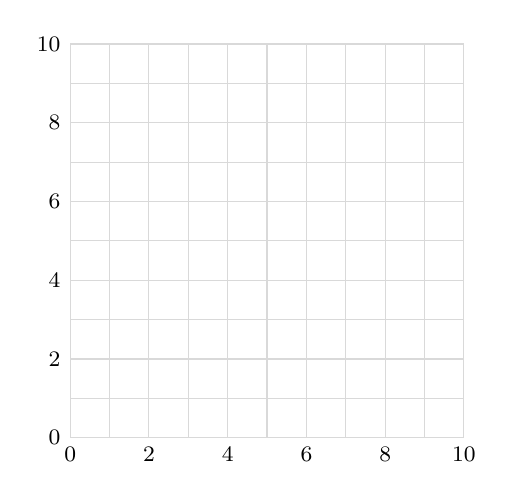
\begin{tikzpicture}[scale=0.5]
  \draw[step=1,gray!30,thin] (0,0) grid (10,10);
  \foreach \x in {0,2,...,10} \node[below] at (\x,0) {\footnotesize $\x$};
  \foreach \y in {0,2,...,10} \node[left] at (0,\y) {\footnotesize $\y$};
\end{tikzpicture}
\end{center}
\end{questionText}
\correctAnswer{Side length $= 6$ units}
\explanation{$\sqrt{36} = 6$. A $6 \times 6$ square has area $36$ square units.}
\end{practiceQuestion}

\begin{practiceQuestion}{3-9-q30}{gsa}
\begin{questionText}
The diagram shows two squares.

\begin{center}
\begin{tikzpicture}[scale=0.4]
  % Square A
  \fill[funBlue!20] (0,0) rectangle (5,5);
  \draw[thick,funBlue] (0,0) rectangle (5,5);
  \node at (2.5,2.5) {A: $25$ sq in};
  % Square B
  \fill[funRed!20] (7,0) rectangle (16,9);
  \draw[thick,funRed] (7,0) rectangle (16,9);
  \node at (11.5,4.5) {B: $81$ sq in};
\end{tikzpicture}
\end{center}

What is the difference between the side lengths of Square B and Square A?
\end{questionText}
\correctAnswer{$4$ inches}
\explanation{Side of A $= \sqrt{25} = 5$ in. Side of B $= \sqrt{81} = 9$ in. Difference: $9 - 5 = 4$ in.}
\end{practiceQuestion}
